\section{Prestudy}
\subsection{Development methods}
\subsubsection{Scrum}
Scrum is an iterative and incremental development framework for development of complex information systems. The use of Scrum requires the team to be divided into specific roles, where each role has its own responsibility. The following is the core roles of the Scrum team:
\begin{description}
	\item[Product owner:]{The product owner represents the stakeholders in the project, and is the voice of the customer. It is the product owner’s responsibility to ensure that the Scrum team at all times is working with the right things seen from a business perspective.}
	\item[Scrum master:]{The scrum master should act as a buffer between the development team and distracting influences, so that the development team can deliver potentially shippable products at the end of each sprint. The scrum master should keep the development team focused at all times.}
	\item[Development team:]{The development team is made up from three to nine persons with cross-functional skills. This team does the all the actual work, including development, testing, designing and so on.}
\end{description}

\subsubsection{Spiral model}
The spiral model is software development model intended for large and complicated projects. It combines elements from the waterfall model and prototyping models, and uses an iterative approach. Based on this it allows for incremental releases of the product.

\subsubsection{Lean sotfware development}
Lean is an agile software development methodology that is defined by seven principles:
\begin{description}
	\item[Eliminate waste.]{Everything that does not add any value to the customer is considered a waste.}
	\item[Amplify learning Defects.]{Should be prevented by running early after the code is made.}
	\item[Decide as late as possible.]{Better result should be achieved with an option-based approach. Delaying options as much as possible would give more flexibility later.}
	\item[Deliver as fast as possible.]{The sooner the product is delivered, the sooner feedback can be received.}
	\item[Empower the team.]{The managers are taught how to listen to the developers, so they can explain better what action that might be taken, and give suggestion for improvement.}
	\item[Build integrity.]{The customer needs to have more influence and inspection of the project.}
	\item[See the whole.]{Decompose the system into smaller parts and find and eliminate defects.}
\end{description}

\subsection{Existing solutions}
This is a summary of existing solutions similar to the project assignment. This section is divided in two subsections; one for the market application and one for the over-the-air transfer. The existing products were evaluated on the following criteria:
\begin{itemize}
	\item{To what degree the product fits the assignment.}
	\item{Can the product, or parts of it, be reused for the assignment? Can it lead to licensing issues?}
\end{itemize}

\subsubsection{Market application}
A prior project created an universal app store in PHP. Had potential for serving as a back end.

{\bf Google Play} is a similar market application for android that categorizes the applications and have a search option. It also detects what model of phone that is being used, and only shows apps that are supported by that phone. The applications are shown in lists and can be downloaded by two clicks. The first click guides you to a description section with pictures, description, comments and user-feedback in form of 5-star-rating.\\
The store is not open source and can only be a source of inspiration for this project.
\begin{figure}[H]
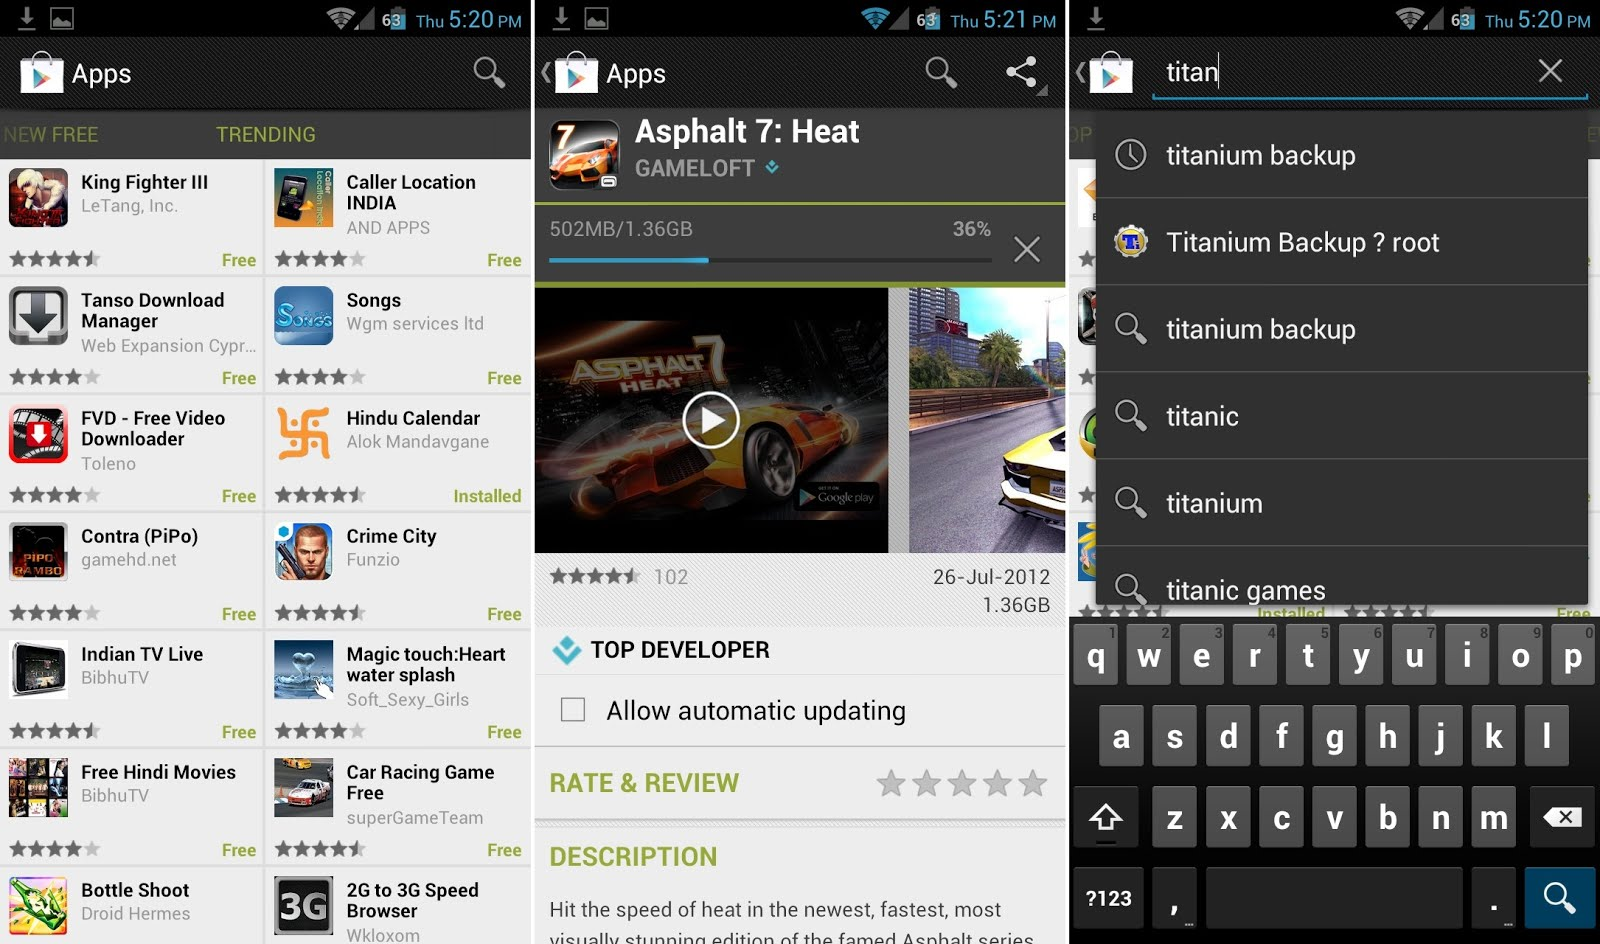
\includegraphics[scale=0.2]{images/Google-Play-Store-APK-3-7-15.jpg}
\caption{Google Play Store}
\end{figure}

{\bf App Store} is also a similar market application, but for apple products\ldots etc\ldots\\
\begin{figure}[H]
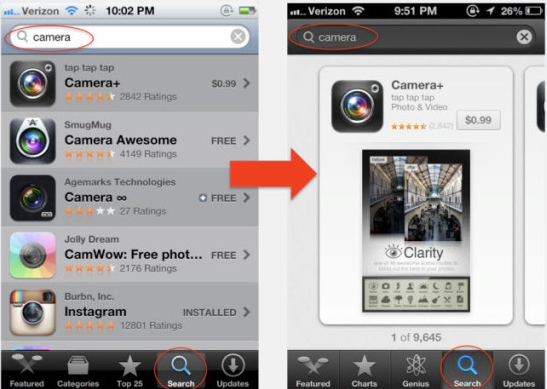
\includegraphics[scale=0.7]{images/png;base642dee0c596030bc1e.png}
\caption{App Store}
\end{figure}
These applications fit the assignment in the way that they are both market applications where one can download applications. This was useful for the development of the product, since it was possible to use the same principles in the assignment. It was also similar in the way that it was possible to browse for applications on the computer, and ''push'' the app to a mobile telephone. This, however, did not connect via bluetooth which the task assignment stated that the finished product should. Based on this, it was not possible to reuse the code or other parts of any of the applications in the development. 

\subsubsection{Over the air transfer}
Pebble is a watch that offers over the air transfer of applications. It is based on the same microchip as one of the newest Arduino\#, but contains an operating system written in C.
\begin{figure}[H]
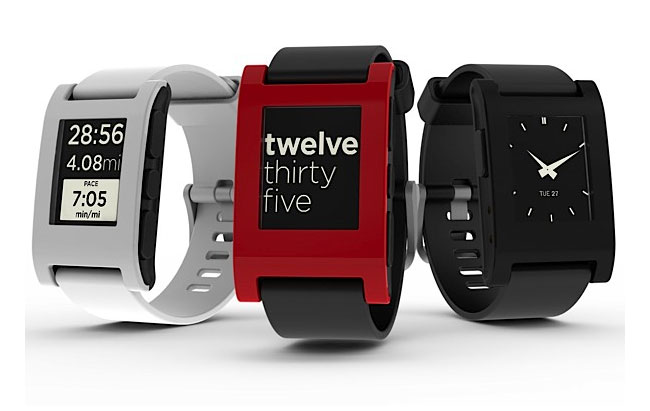
\includegraphics[scale=0.7]{images/Pebble-Smartphone-Watch.jpeg}
\caption{Pebble Watch}
\end{figure}
There was very little documentation on the Pebble website, so the potential reuse in this project appears minimal.